\documentclass[12pt]{article}
\usepackage[portuguese]{babel}
\usepackage{natbib}
\usepackage{url}
\usepackage[utf8x]{inputenc}
\usepackage{amsmath}
\usepackage{graphicx}
\graphicspath{{images/}}
\usepackage{parskip}
\usepackage{fancyhdr}
\usepackage{vmargin}
\setmarginsrb{1.5 cm}{2 cm}{1.5 cm}{1 cm}{1 cm}{1.5 cm}{1 cm}{1.5 cm}

\title{Assignment 4}								% Title
\author{ME19B089-Bukya Gopi Chand Naik}								% Author
\date{\today}											% Date

\makeatletter
\let\thetitle\@title
\let\theauthor\@author
\let\thedate\@date
\makeatother

\pagestyle{fancy}
\fancyhf{}
\rhead{\theauthor}
\lhead{\thetitle}
\cfoot{\thepage}

\begin{document}

%%%%%%%%%%%%%%%%%%%%%%%%%%%%%%%%%%%%%%%%%%%%%%%%%%%%%%%%%%%%%%%%%%%%%%%%%%%%%%%

\begin{titlepage}
	\centering
    \vspace*{0.1 cm}
    
\includegraphics[scale = 0.25]{iitm.jpg}\\[1.0 cm]	% University Logo
    \textsc{\LARGE Indian Institute of technology}\\ [0.5 cm]% University Name
    \textsc{\LARGE MADRAS} \\ [2.0 cm]
	\textsc{\Large ID2090: introduction to scientific computing}\\[0.5 cm]				% Course Code
	\rule{\linewidth}{0.3 mm} \\[0.4 cm]
	{ \huge \bfseries \thetitle}\\
	\text\newline\newline\large  {ME19B089-BHUKYA GOPI CHAND NAIK}
	\rule{\linewidth}{0.2 mm} \\[0.5 cm]
	\text{26th july 2021}
	
    \end{titlepage}

%%%%%%%%%%%%%%%%%%%%%%%%%%%%%%%%%%%%%%%%%%%%%%%%%%%%%%%%%%%%%%%%%%%%%%%%%%%%%%%%%%%%%%%%%

\newpage

\begin{center}
\textsc{\LARGE Mass-Energy Equation:} \\ [1.0 cm]
\huge \huge \bfseries \boxed{E=mc^2}\\[1.5 cm]
\end{center} 
\large{\textit{Einstein's Energy-Mass Equivalence:}}\\ [0.5 cm]
Mass–energy equivalence states that all objects having mass, have a corresponding intrinsic energy, even when they are stationary. In the rest frame of an object, where by definition it is motionless and so has no momentum, the mass and energy are equivalent and they differ only by a constant, the speed of light squared (c$^2$).\\ [0.3 cm]
In Newtonian mechanics, a motionless body has no kinetic energy, and it may or may not have other amounts of internal stored energy, like chemical energy or thermal energy, in addition to any potential energy it may have from its position in a field of force. These energies tend to be much smaller than the mass of the object multiplied by c$^2$, which is on the order of 1017 joules for a mass of one kilogram. Due to this principle,\textit{the mass of the atoms that come out of a nuclear reaction is less than the mass of the atoms that go in, and the difference in mass shows up as heat and light with the same equivalent energy as the difference.}\\ [0.3 cm]
\begin{figure} [h!]
    \centering
    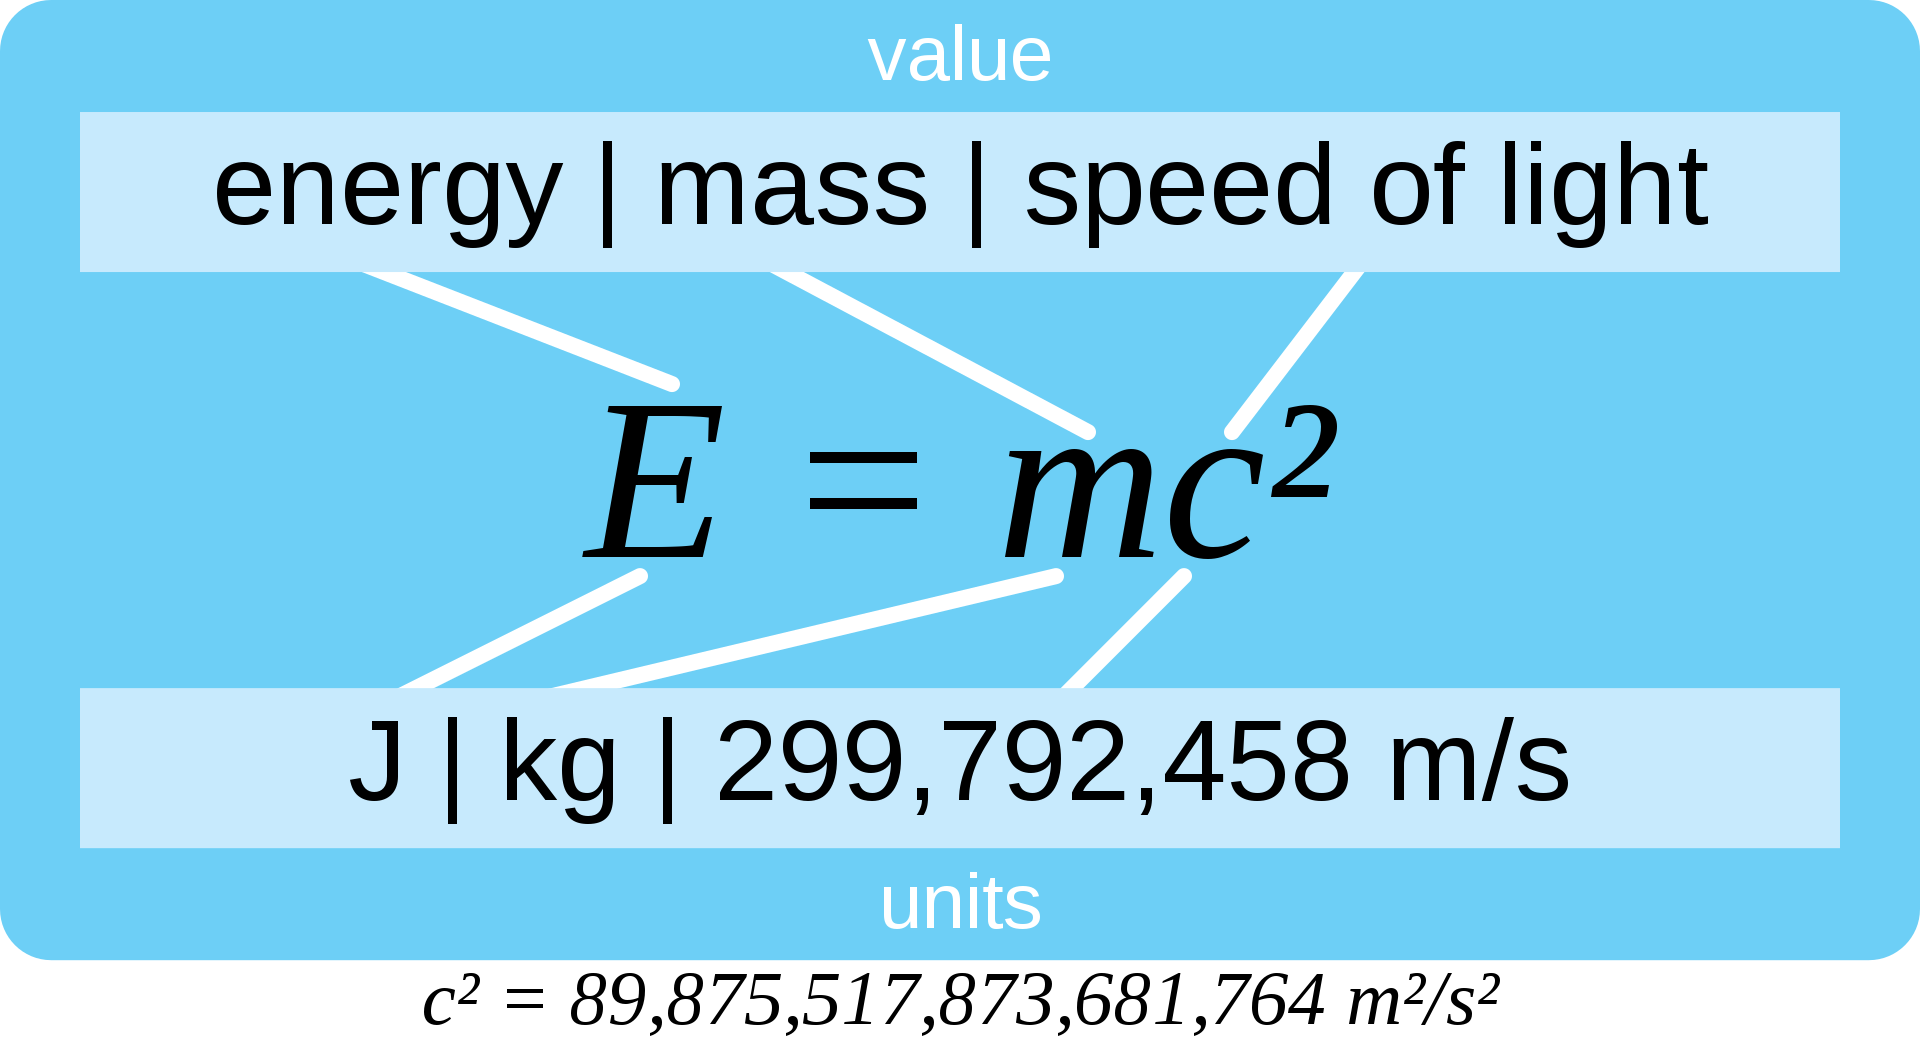
\includegraphics[scale = 0.20]{10.png}
\end{figure} \\[0.3 cm]
In analyzing these explosions, Einstein's formula can be used with E as the
energy released and removed, and m as the change in mass.\\[0.3 cm]
In relativity, all the energy that moves with an object (\textit{i.e.,} the energy as measured in the object's rest frame) contributes to the total mass of the body, which measures how much it resists acceleration. If an isolated box of ideal mirrors could contain light, the individually mass-less photons would contribute to the total mass of the box, by the amount equal to their energy divided by c$^2$.\\[0.3 cm]
For an observer in the rest frame, removing energy is the same as removing mass and the formula m = E/c$^2$ indicates how much mass is lost when energy is removed.In the same way, when any energy is added to an isolated system, the increase in the mass is equal to the added energy divided by c$^2$.\\[0.3 cm]
The biggest impact of this equation and perhaps the event that secured its legacy was the development and subsequent use of atomic bombs at the end of WW-2. These bombs horrifically demonstrated the extraction of a huge amount of energy from a tiny amount of mass.\\

\begin{figure} [h!]
    \centering
    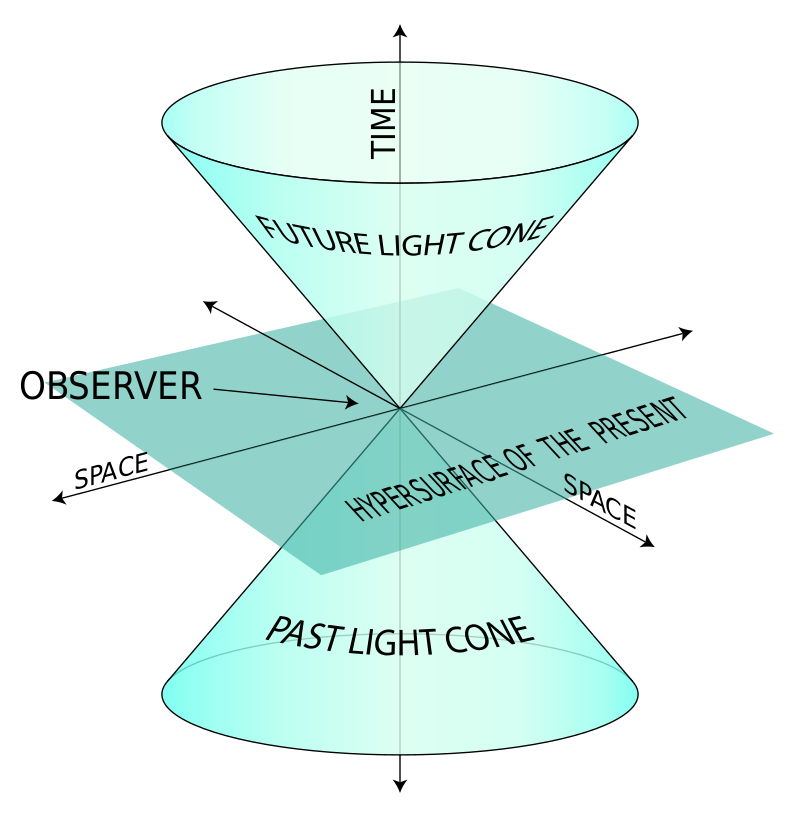
\includegraphics[scale = 0.3]{20.png}
\end{figure}
\centering
	\rule{\linewidth}{0.3 mm} \\[0.4 cm]
	{ \huge \bfseries Thank You!}\\
	\rule{\linewidth}{0.2 mm} \\[0.5 cm]
\end{document}